\chapter{Soporte de Turtlebot 2 en ROS Foxy}
\label{cap:capitulo4}

% -- INTRODUCCION
% -----------------
En este capítulo se presenta el proceso de \textbf{migración} del robot Turtlebot 2 de ROS Noetic a \textbf{ROS Foxy}. Se describirán todos los cambios relevantes realizados como puede ser la modificación de sus ficheros URDF/XACRO, su lanzamiento en Gazebo a través de los launchers de ROS2 o incluso su integración sobre una imagen Docker.\\

El soporte más estable del Turtlebot 2 se encuentra en la rama de \textbf{ROS Melodic} (tanto real como simulado) aunque también funciona en ROS Noetic \footnote{\textbf{Turtlebot 2 (Noetic)}: \url{https://bitbucket.org/theconstructcore/turtlebot/src/noetic/}}. Sin embargo, para ROS 2 Foxy solamente hay un repositorio \footnote{\textbf{Base Kobuki (foxy)}: \url{https://github.com/kobuki-base/kobuki_ros}} con los drivers para mover la base kobuki [\ref{sec:kobuki_base}] real (sin  ficheros de lanzamiento para Gazebo).\\

De modo que el \textbf{primer paso} del TFG era dar soporte completo al Turtlebot 2 en ROS Foxy para poder desarrollar los nuevos ejercicios de Robotics Academy. A continuación mostraré en orden los pasos realizados hasta su resultado final.\\


% -- SECCION KOBUKI BASE
% ------------------------
\section{Kobuki Base}
\label{sec:kobuki_base}

El respositorio oficial de kobuki base contiene los siguientes paquetes relevantes:

\begin{itemize}
	\item \textbf{kobuki\_description}: Es el paquete que contiene los ficheros de descripción xacro [\ref{sec:xacro}] y URDF [\ref{sec:urdf}] de la base. Con este directorio se describe el \textbf{árbol de tranformadas} que existen entre todos los links del robot, y de esta manera poder conocer la localización de todos los frames. También se añaden plugins para facilitar el control de movimiento del robot (controladores de velocidad, odometría ...).
	\item \textbf{kobuki node}: Es el paquete que contiene un fichero de configuración denominado \textbf{kobuki\_node\_params.yaml} con el que podemos conectarnos al robot real usando el puerto \textbf{/dev/ttyUSB0}, así como la definición de algunos frames (base, odom). También contiene los ficheros de los nodos necesarios para controlar la base kobuki y su odometría. Oculta al programador la complejidad de comunicarnos directamente con el hardware (motores, leds...) del robot usando nodos ros con publicadores y suscriptores. El nodo que lanza \textbf{kobuki\_ros\_node} se suscribe al tópic \textbf{/commands/velocity} para recibir mensajes de tipo \textbf{geometry\_msgs.msg.Twist} y poder mover mediante velocidad lineal y angular la base del robot. Este directorio no tiene relación con kobuki\_description.
	\item \textbf{kobuki\_keyop}: Es un paquete que nos permite mover la base del robot con el teclado del ordenador. Se crea un nodo que publica por cada pulsación del teclado, un mensaje \textbf{geometry\_msgs.msg.Tiwst} en el topic \textbf{/cmd\_vel} (tendremos que cambiar a \textit{/commands/velocity} si queremos controlar el robot real. Este paquete nos puede ayudar en un principio a comprobar que tenemos conexión con el hardware real.
\end{itemize}

Con estos 3 paquetes tenemos lo necesario para controlar la base del robot. Sin embargo, solo nos sirve para el robot real, y no en simulado. Como se ha mencionado antes, el paquete \textbf{kobuki\_description} no tiene relación con kobuki\_node, solo nos permite visualizar un árbol de transformadas con el visualizador \textbf{RVIZ 2} de modo que el siguiente paso fue representar la base kobuki, mediante los ficheros de descripción, en un escenario de Gazebo.\\




% -- SECCION LANZAMIENTO EN GAZEBO
% ----------------------------------
\subsection{Lanzamiento en Gazebo}
\label{subsec:kobuki_gazebo}

Para conseguir la representación de la base kobuki en Gazebo hice un \textbf{fork}\footnote{\textbf{Kobuki ROS (fork)}: \url{https://github.com/Carlosalpha1/kobuki_ros}} del repositorio oficial e implemente un nuevo paquete llamado \textbf{kobuki\_gazebo}. Dentro incluí ficheros \textbf{launch.py} para lanzar tanto el simulador Gazebo como la base kobuki simulada. A continuación describiremos los ficheros más importantes del nuevo paqueté implementado:

\begin{itemize}
	\item \textbf{empty\_world.launch.py}: Un punto de partida en muchas ocasiones cuando creamos un robot simulado es diseñar un fichero de lanzamiento que únicamente lance un mundo vacío en Gazebo. De esta manera, puedes incluir ese fichero en otros ficheros de lanzamiento y dividimos un problema complejo en varios subproblemas. Para lanzar \textbf{Gazebo} en ROS 2 ejecutamos 2 ficheros de lanzamientos en este orden:
	\begin{enumerate}
		\item \textbf{gazebo\_ros - gzserver.launch.py}: Lanza un servidor gazebo sin ventana, de modo que podemos ejecutar programas sin necesidad de visualizar el resultado en Gazebo.
		\item \textbf{gazebo\_ros - gzclient.launch.py}: Lanza un cliente gazebo que activa una ventana donde podemos ver el mundo solicitado.
	\end{enumerate}
	
	\cleardoublepage
\begin{code}[H]
\begin{lstlisting}[frame=single]
def generate_launch_description():

	ld = LaunchDescription()

	pkg_gazebo_ros = get_package_share_directory('gazebo_ros')
		
	gazebo_server = IncludeLaunchDescription(
		PythonLaunchDescriptionSource(os.path.join(pkg_gazebo_ros, 'launch', 'gzserver.launch.py'))
	)
		
	gazebo_client = IncludeLaunchDescription(
		PythonLaunchDescriptionSource(os.path.join(pkg_gazebo_ros, 'launch', 'gzclient.launch.py'))
	)
	
	ld.add_action(gazebo_server)
	ld.add_action(gazebo_client)
	
	return ld
\end{lstlisting}
\caption[kobuki\_gazebo: empty\_world.launch.py]{kobuki\_gazebo: empty\_world.launch.py}
\label{cod:kobuki_gazebo_empty_world}
\end{code}

	\item \textbf{spawn\_model.launch.py}: Este fichero pasa los datos de descripción \textbf{urdf} de la base kobuki a un parámetro denominado \textbf{/robot\_description}, publica el estado del robot, sus transformadas y ejecuta el fichero de gazebo\_ros \textbf{spawn\_entity.py} para visualizar el modelo en el simulador:
	
\begin{code}[H]
\begin{lstlisting}[frame=single]
kobuki_model = Node(
	package='robot_state_publisher',
	executable='robot_state_publisher',
	parameters=[{'robot_description': robot_desc}],
	arguments=[urdf_file]
)

joint_state_publisher_node = Node(
	package='joint_state_publisher',
	executable='joint_state_publisher',
	name='joint_state_publisher'
)

spawn_entity = ExecuteProcess(
	cmd=['ros2', 'run', 'gazebo_ros', 'spawn_entity.py', '-topic', '/robot_description', '-entity', 'kobuki'], output='screen')
\end{lstlisting}
\caption[kobuki\_gazebo: spawn\_model.launch.py]{kobuki\_gazebo: spawn\_model.launch.py}
\label{cod:kobuki_gazebo_spawn_model}
\end{code}
\end{itemize}

Podremos visualizar la base kobuki en simulado ejecutando los siguientes comandos:\\
\begin{lstlisting}
ros2 launch kobuki_gazebo empty_world.launch.py &
ros2 launch kobuki_gazebo spawn_model.launch.py
\end{lstlisting}\

En la figura \ref{fig:sim_kobuki_base} podréis ver el resultado de la base kobuki simulada en Gazebo
\begin{figure} [H]
  \begin{center}
    \includegraphics[width=10cm]{imagenes/sim_kobuki_base.png}
  \end{center}
  \caption[\textbf{Modelo simulado} de Kobuki Base (ROS 2 Foxy)]{\textbf{Modelo simulado} de Kobuki Base (ROS 2 Foxy)}
  \label{fig:sim_kobuki_base}
\end{figure}\




% -- SECCION IMAGEN DOCKER
% --------------------------
\subsection{Imagen Docker}
\label{sec:kobuki_base_docker}

Para empezar a controlar la base kobuki con un contenedor docker, definimos un fichero Dockerfile con todas las dependencias necesarias junto con los comandos necesarios para lanzar los nodos.\\

En esta dirección, podréis descargar una versión de prueba para mover un robot real Turtlebot 2 en ROS Foxy con el paquete \textbf{kobuki\_keyop} sin necesidad de instalar ROS 2 ni ningún otro paquete: \url{https://hub.docker.com/r/carlosalpha1/kobuki_keyop}. Al lanzar el contenedor mostrará una ventana emergente de un terminal \textbf{xterm} para pulsar las teclas correspondientes que moverán la base del robot.\\

\textbf{Comandos para lanzar el contenedor kobuki\_base}:\\
\begin{lstlisting}
xhost +
docker run -it --rm --device /dev/ttyUSB0 -e DISPLAY=$DISPLAY -v /tmp/.X11-unix:/tmp/.X11-unix carlosalpha1/kobuki_keyop:ros-foxy
xhost -
\end{lstlisting}\

Controlar la base kobuki supone un avance muy significativo para poder usar el robot Turtlebot 2. Solamente haría falta usar paquetes de ROS para el láser y la cámara (tal y como veremos en el capítulo [\ref{cap:capitulo6}]). Sin embargo, aún no tenemos disponible la simulación del robot Turtlebot 2 completo, por lo que en los siguientes apartados integraremos la estructura que soporta la base.\\



% -- SOPORTE TURTLEBOT 2
% ------------------------
\section{Soporte Turtlebot 2}
\label{sec:soporte_turtlebot2}

A parte de la base Kobuki, la otra mitad que caracteriza al Turtlebot 2 es la \textbf{base superior} que permite colocar portátiles, sensores o actuadores. En esta sección abordaremos la migración a ROS Foxy de esta última parte del robot.\\

La \textbf{pregunta}, es \textit{¿por qué no usamos ficheros turtlebot\_description de la rama Noetic o Melodic si el lenguaje URDF es el mismo?} En realidad, el paso de ROS 1 a ROS 2 conlleva cambios tanto en la manera de crear nodos, ficheros de lanzamiento y su funcionamiento interno como en el uso de URDF. El modelo Turtlebot 2, al tener una gran cantidad de ficheros URDF que dependían unos de otros, y estos a su vez de otros paquetes con dependencias de ROS 1, no facilitaba la tarea de obtener un modelo creando únicamente ficheros launch.py como hicimos con la base kobuki.\\

Entonces, la \textbf{solución} fue crear la estructura restante del robot a mano, usando la sintáxis URDF y XACRO, creando un modelo lo más semejante posible al real. A continuación mostraré las fases del desarrollo. Una vez terminado el modelo Turtlebot 2 simulado, tendremos por un lado un directorio con todos los paquetes de kobuki\_base y otro directorio con la definición del nuevo soporte creado.\\



% -- FICHEROS DE CONFIGURACION XACRO
% ------------------------------------
\subsection{Ficheros de Configuración XACRO}
\label{sec:turtlebot2_xacro}

El primer paso de esta segunda parte fue crear el modelo URDF. Usando XACRO me permitió crear \textbf{macros} que facilitara la estructura y la legibilidad del modelo. Con XACRO era sencillo incluir nuevos elementos en el modelo y establecer la jerarquía de transformadas entre links de padres a hijos (siempre es importante indicar las relaciones jerárquicas para poder realizar futuras operaciones basadas en frames).\\

La estructura del nuevo directorio es la siguiente:
\begin{figure}[H]
	\begin{center}
	    \setlength{\fboxsep}{0.5cm}
	    \fbox{
        \begin{minipage}{10cm}
          \dirtree{%
          .1 turtlebot2.
          .2 kobuki\_base.
          .3 kobuki\_ros\_interfaces.
          .3 kobuki\_ros.
          .4 Ficheros de kobuki\_gazebo \ref{sec:kobuki_gazebo}.
          .4 \vdots.
          .2 turtlebot2.
          .3 launch.
          .4 empty\_world.launch.py.
          .4 spawn\_model.launch.py.
          .3 rviz.
          .3 urdf.
          .4 structures.urdf.xacro.
          .4 colors.urdf.xacro.
          .4 turtlebot2.urdf.xacro.
          .4 sensors.
          .5 camera.urdf.xacro.
          .5 lidar.urdf.xacro.
          .3 spawn.sh.
          .3 CMakeLists.txt.
          .3 package.xml.
          }
        \end{minipage}
        }
	    \caption{Estructura de directorios completa del Turtlebot 2 (ROS 2 Foxy)}
	    \label{fig:directorios_turtlebot2}
	\end{center}
\end{figure}\

En el fichero \textbf{colors.urdf.xacro} definimos algunas macros para establecer colores en el modelo de gazebo:\\
\begin{code}[H]
\begin{lstlisting}
<xacro:macro name="create_color" params="name value">
	<material name="${name}">
		<color rgba="${value}"/>
	</material>
</xacro:macro>

<xacro:macro name="gazebo_color" params="link color">
	<gazebo reference="${link}">
		<material>Gazebo/${color}</material>
	</gazebo>
</xacro:macro>

<xacro:create_color name="Gray" value="0.5 0.5 0.5 1"/>
<xacro:gazebo_color link="base_tick1_link" color="Gray"/>
\end{lstlisting}
\caption{Creación y establecimiento de un color a un \textbf{link}}
\label{fig:creacion_color_link}
\end{code}\

En el fichero \textbf{structures.urdf.xacro} definimos 2 macros para crear los links que necesitamos y definimos las \textbf{relaciones jerárquicas} de padres a hijos. Las nuevas macros son \textbf{cylinder\_structure} y \textbf{cube\_structure}, para crear en el fichero turtlebot2.urdf.xacro elementos como los siguientes:
\begin{code}[H]
\begin{lstlisting}
<xacro:cylinder_structure name="base_tick5" x="0.15" y="0.0" z="0.14" length="0.15" radius="0.005" parent="base_link"/>
<xacro:cube_structure name="camera_support_base" x="0.13" y="0" z="0.0975" x_size="0.0175" y_size="0.15" z_size="0.005" parent="middle_base_link"/>
\end{lstlisting}
\caption{Creación de 2 links usando 2 nuevas macros definidas}
\label{fig:creacion_link_macro}
\end{code}\

En el fichero turtlebot2.urdf.xacro incluimos con la macro \textbf{xacro:include} las definiciones URDF de los ficheros del paquete \textbf{kobuki\_description}. Por último, creamos dos ficheros XACRO para colocar una cámara RGBD y un láser 360 grados. Los ficheros de los sensores los podéis ver en este \textbf{enlace}. \footnote{\textbf{Sensores Turtlebot2}: \url{https://github.com/RoboticsLabURJC/2021-tfg-carlos-caminero/tree/main/turtlebot2/turtlebot2/urdf/sensors/}}\\

Mediante este comando podemos generar un fichero urdf con toda la descripción del modelo a partir de turtlebot2.urdf.xacro:\\
\begin{lstlisting}
ros2 run xacro xacro urdf/turtlebot2.urdf.xacro > urdf/turtlebot2.urdf
\end{lstlisting}\




% -- TURTLEBOT 2: LANZAMIENTO EN GAZEBO
% ---------------------------------------
\subsection{Lanzamiento en Gazebo}
\label{sec:turtlebot2_gazebo}

Para la \textbf{visualización} del modelo URDF en Gazebo me basé en los mismos ficheros que hice con la base Kobuki: \textbf{empty\_world.launch.py} y \textbf{spawn\_model.launch.py} [\ref{sec:kobuki_gazebo}]\\

La única diferencia fue definir 3 argumentos por defecto para establecer la \textbf{posición inicial} del robot, para que cuando se quiera importar el modelo en cualquier otro mundo de Gazebo, el programador pueda especificar el punto de inicio. Estos 3 argumentos se pasan al nodo \textbf{spawn\_entity}. A continuación podemos ver la sección referente a la posición inicial del fichero \textbf{spawn\_model.launch.py}:\\
\begin{lstlisting}
	# Set (x, y, z) default position of turtlebot2
	x_pos = LaunchConfiguration('-x', default='0')
	y_pos = LaunchConfiguration('-y', default='0')
	z_pos = LaunchConfiguration('-z', default='0')
	
	spawn_entity_node = Node(
		package='gazebo_ros',
		executable='spawn_entity.py',
		name='entity_spawner',
		output='screen',
		arguments=["-topic", "/robot_description", "-entity", "turtlebot2", "-x", x_pos, "-y", y_pos, "-z", z_pos]
	)
\end{lstlisting}\

Una vez abierto Gazebo, para lanzar el modelo ejecutamos el siguiente comando:\\
\begin{lstlisting}
ros2 launch turtlebot2 spawn_model.launch.py
\end{lstlisting}\

En la figura \ref{fig:evolucion_turtlebot2_sim} podemos ver la evolución del proceso creativo del Turtlebot 2 simulado:
\begin{figure} [H]
  \begin{center}
    \includegraphics[width=10cm]{imagenes/creacion-turtlebot2-sim.png}
  \end{center}
  \caption[Evolución Turtlebot 2 simulado]{Evolución Turtlebot 2 simulado}
  \label{fig:evolucion_turtlebot2_sim}
\end{figure}\


\textbf{Consideraciones a tener en cuenta}: Tanto el modelo Kobuki como el Turtlebot 2 simulado usan un plugin para controlar los motores denominado \textbf{differential\_drive\_controller.so}. Este plugin se suscribe a un topic para controlar la velocidad de las ruedas del robot llamado \textbf{/cmd\_vel} (estándar en ROS), por lo que no coincide con el topic del robot real \textbf{/commands/velocity}.


